\chapter{Feladat megvalósítása}
\label{ch:imp}
Mint már fentebb említésre került, a dolgozat témája részben egy valós, határidős projekt volt, így ennek megfelelően egy csapat dolgozott rajta. Ezen belül én is részfeladatokat kaptam és implementáltam, valamint részt vettem a tervezési procedúrában. 

\section{Wrapper fejlesztése QRadar-hoz}
A projekt első kihívása egy Java alapú wrapper fejlesztése volt a QRadar reference data manipulációt kezelő webes REST apijához. Későbbiekben ezen a wrapperen keresztül bonyolítunk majd minden forgalmat az átláthatóbb kód készítése céljából, ezért fontos hogy a wrapper megvalósítson minden olyan funkciót amire szükség lehet.

A fejlesztés első lépéseként tanulmányoztam a REST Api-hoz tartozó referencia dokumentációt, ami leírja mely endpointokon milyen HTTP kérések hajthatók végre, milyen paraméterekkel, milyen választ adhat és milyen státusz üzeneteket kaphatunk. Ebből az anyagból kiderült, hogy a négy reference data típushoz 4 endpoint halmaz tartozik, amelyek hasonló felépítéssel és paraméterezéssel bírnak. Egy ilyen endpoint halmazra mutat példát az alábbi felsorolás.

\begin{itemize}
	\item /sets - GET, és POST műveletet támogat. A POST-tal új reference set hozható létre, a GET metódussal pedig lekérhető a rendelkezésre álló setek listája.
		\subitem /\{name\} - GET, POST, DELETE. Az URL-ben megadott paramétert a QRadar a reference set neveként értelmezi, és ezen keresztül érhető el a set lekérése (GET), teljes törlése (DELETE), valamint egy elemi adat feltöltése (POST).
			\subsubitem /\{value\} - DELETE. Ennek az endpointnak a segítségével tudunk egy bizonyos értéket törölni a reference set-ből.
		\subitem /bulk\_load/\{name\} - POST. Az egyik legfontosabb endpoint, mivel ezen keresztül tudunk feltölteni egy olyan JSON formátumú szöveget, amellyel egyszerre több értéket is tudunk állítani egy reference set-ben (vagy más endpointok esetén más reference data-kban).
\end{itemize}

A fent felsorolt endpointok közül mindegyiket implementáltam a wrapperben, Java konvención alapuló neveket adva  a függvényeknek. Egy függvény egy működést valósít meg, és ez a működés a reference data típusának szempontjából transzparens, tehát nem szükséges külön metódust hívni egy reference set és egy reference map feltöltéséhez, hanem elég egy metódust, más paraméterekkel.

A reference data-kkal való könnyebb interakció miatt definiáltunk egy saját adatszerkezetet egy Java osztály formájában, a data típusokkal megegyező néven. Mindegyik osztály egy ReferenceData navű absztrakt ősosztályból származik, ami egy egységes interface-t biztosít a leíró adatok, mint például a típus, az adatok típusa, lekéréséhez. Ennek a ReferenceData-nak a leszármazottai a konkrét reference típusokat megvalósító osztályok. Mindegyik osztály rendelkezik egy, a saját maga által reprezentált struktúrának megfelelő tárolóval, amely tárolja az adott reference data adatait. Mivel az integráció során többnyire szöveges, vagy azzá könnyen átalakítható adatokkal dolgozunk, és a QRadar irányába is JSON formátumban továbbítjuk az adatokat, így kézenfekvő mindet szövegként tárolni. A tárolókhoz használt kollekciók pontos típusa, valamint az implementációhoz használt architektúra leolvasható a mellékelt ábráról \ref{fig:referencedata}. 

Lehetséges lenne más formátumban tárolni az adatokat, mint például egy Java alapú JSON reprezentációban, JSONObject-ben, vagy akár egy hosszú karakterláncként is, ám ezzel elvesztenénk a Java beépített kollekciói által nyújtott funkciókat, mint például az iterációt, vagy a tartalmazás ellenőrzését. Ezek mind nélkülözhetetlen funkciók a könnyű fejlesztés érdekében, valamint a megfelelő teljesítmény biztosítása szempontjából is fontosak, amire később látunk majd példát. 

\begin{figure}
	\centering
	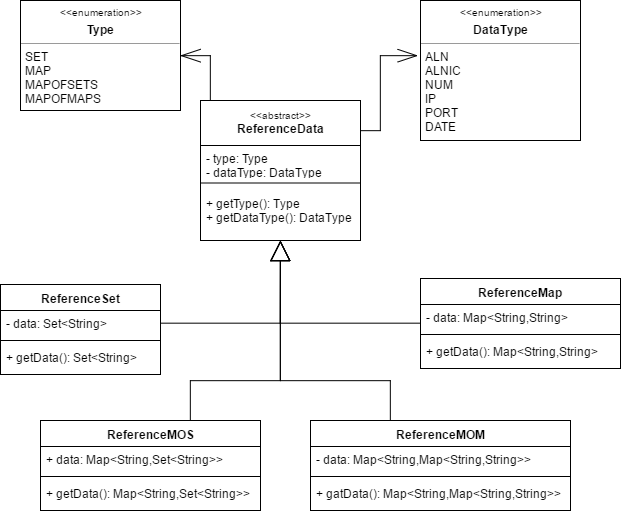
\includegraphics[width=0.7\linewidth]{figures/ReferenceData}
	\caption{A ReferenceData osztály és leszármazottainak felépítése}
	\label{fig:referencedata}
\end{figure}

A wrapper fejlesztése közben külön kihívást jelentett a QRadar REST api-val való kommunikáció megvalósítása. A QRadar ugyanis csak HTTPS forgalmat fogad el, TLS segítségével, ezért egy, a QRadar által generált tanusítványt kellett hozzáadni minden olyan környezethez, amely a wrappert használta. Ez a két külön architektúra esetén a WebSphere és a TDI tanusítvány könyvtárát jelentette, és ez egy olyan követelmény, ami a wrapper későbbi használata esetén is szükséges. Emellett a QRadar megköveteli, hogy a REST API-jához csatlakozó kliensek használjanak egy, a QRadar által előre generált token-t, amit minden híváskor fel kell küldeniük. A wrapper osztály ezt konstruktorában kéri, és automatikusan minden kérésnél elküldi. A TLS kapcsolat biztosítja a szerver hitelességét, míg a token a szerver számára hitelsíti az API-t használó klienst, így összeségében a kommunikáció kölcsönösen hitelesített.

Magának a HTTP forgalomnak és a REST hívásoknak a lebonyolítására az Apache Wink\footnote{\hyperlink{Apache Wink}{\url{https://wink.apache.org}}} framework-öt használtam. Ez egy egyszerű Java alapú framework, melynek része egy JAX-RS kompatiblis szerver, és egy kifejezetten REST hívások lebonyolítására kiélezett HTTP kliens. A projektben a kliens komponens RestClient osztályát használtam, valamint a frameworkkel együtt érkező JSON4J csomagot, a JSON inputok parse-olására és a szöveges outputok generálására. A fejlesztés közben külön kihívást jelentett a JSON4J csomag megfelelő osztályainak használata, valamint egymásba ágyazása. Ez a csomag ugyanis két osztályt bocsájt rendelkezésre a JSONObject valamint a JSONArray formájában. Az object osztály reprezentálja a map típusú, míg az array a tömb típusú struktúrákat. Ez annyiban nehezítette a fejlesztést, hogy a különböző ReferenceData leszármazottak közt nem lehetett egységes parseolást használni, hanem a többszörösen egymásba ágyazott kollekciók esetén több lépcsős iterációt kellett használni a JSON felépítéséhez. Ez túl nagy adathalmazoknál lassabb működést eredményezhet.

A wrapper a különböző reference data-k transzparens kezelésén túl egyéb funkciókat is ellát, mint például segéd funkciók biztosítása, vagy a hibák egységes kezelése. Ilyen segéd funkciók a különböző adattranszformációk a használt típusok és a JSON formátum között, vagy például különböző ellenőrzések egy reference data létezésére, vagy egy aszinkron törlés lefutására. A hibakezelés menedzselésére a wrapper egy saját kivétel osztályt definiál, ami minden, a sikeres lefutástól eltérő esetben (akár belső hiba, akár a QRadarral való kommunikáció közben fellépő hiba) eldobásra kerül. Ez az objektum tartalmaz egy szöveges üzenetet, ami a hiba okára utal, valamint egy státusz kódot, ami ha HTTP kommunikáció közbeni hiba történt, annak a kódját tartalmazza, ha belső működésbeli hiba (például parse-olási hiba) akkor egy 0-nál kisebb számot tartalmaz. Ez egységesen és könnyen használhatóvá teszi a felsőbb rétegek számára, ahol például logolást kezeljük, mert egyértelmű, hogy a hiba milyen forrásból adódott. A saját kivétel típus pedig tovább könnyíti a hibák elválasztását, főleg ha a wrapper-t egy nagyobb framework-ben használjuk.

\section{TDI Integráció megvalósítása}
% Mod
A TDI alapú megoldás célja egy olyan keret, és hozzá tartozó proof of concept use case-ek kidolgozása, amely lehetőséget ad az ISIM és QRadar közti integrációs feladatok gyors, hatékony és egyszerű megvalósítására. Mivel a TDI által nyújtott keretrendszerbe illeszkedik a megoldás, így képes használni az általa nyújtott számos lehetőséget, például a már létező connector-okat sokféle rendszerhez, valamint a use case implementációk alapján később könnyedén készíthetők új megoldások olyanok által, akik járatosak a TDI használatában. 

A megvalósításhoz szükség volt elsősorban egy connector létrehozására, majd ezt felhasználva implementáltam néhány tényleges megoldást, általunk, valamint az ügyfél által definiált esetekre.
% Mod
 
\subsection{QRadar connector fejlesztése TDI-hoz}
A projekt következő lépése a connector fejlesztése volt a TDI és a QRadar közti integrációhoz. Ehhez segítségemre volt a hivatalos útmutató\footnote{\url{https://www.ibm.com/support/knowledgecenter/SSCQGF_7.1.1/com.ibm.IBMDI.doc_7.1.1/referenceguide177.htm}} connector fejlesztéshez, ami az IBM oldalán megtalálható. Egy saját connector fejlesztése TDI alatt abból áll, hogy létrehozunk egy új Java osztályt ami implementálja a megfelelő, TDI által specifikált interfészt, ennek metódusain belül elkészítjük a kívánt üzleti logikát, majd egy xml leíró fájllal együtt, a megfelelő struktúrában becsomagoljuk azt egy JAR fájlba, amit a TDI által használt könyvtárak egyikébe másolunk. 

Alapvetően hat működési módja lehet egy connector-nak, amit a feljebb említett dokumentum specifikál. Ezek a következők:

\begin{itemize}
	\item Iterator - Végigiterál az adatforrás elemein, azokat felolvassa, és az assembly line rendelkezésére bocsájtja.
	\item AddOnly - Az assembly line-on érkező adatokat hozzáadja az adatforráshoz.
	\item Lookup - Lehetőséget ad több adatforrás elemeinek illesztésére. Úgynevezett link criteria megadásával az erre illeszkedő elemeket választja ki.
	\item Delete - Az assembly line-ról kapott összes elem esetén a megadott link criteria-t felhasználva megpróbálja megkeresni az elemet, és ha megtalálta, törli azt. Lehetőség van olyan felparaméterezésre is, amely egyszerre több elemet töröl.
	\item Update - Már meglévő adatok módosítását végzi. Előbb megpróbálja megkeresni a link criteria-val megadott rekordokat, ha talált ilyen elemet, akkor összehasonlítja az assembly line-on érkező elemmel, és elvégzi a szükséges módosításokat. Ha nem talált megfelelő elemet, akkor hozzáadja újként.
	\item Delta - Egy különleges mód, melyhez szükség van további, ilyen módot támogató elemekre az assembly line-on. A felolvasott adatokat összehasonlítja egy külső tárolóban (ún. delta store) tárolt elemekkel, és a két elem differenciáiból delta műveleteket képez, amiket végrehajt a célrendszeren. Lényegében eltárolja a kezelt elemek legutóbb használt verzióját, és csak az újonnan beolvasott elemekhez képesti különbséget hajtja végre.
\end{itemize}

Ezek a módok meghatározzák, hogy a fejlesztendő connector-nak milyen metódusokat muszáj implementálnia a megfelelő működéshez. Például az AddOnly mód csak az Initialize, putEntry, és a terminate metódusokat használja, így ha a connector csak ezt akarja használni, elég ezeket implementálni. Ezzel szemben például az Update mód ezeken felül használja a findEntry, és a modEntry metódust is. Minden connector a saját logikáját definiálja, amivel megvalósítja az adott célrendszeren az absztrakt módon megfogalmazott műveletet. Egy JDBC connector például adatbázis parancsokkal valósítja meg a fent definiált műveleteket egy kapcsolaton keresztül. Jelen esetben egy REST API-n keresztül elérhető a kommunikáció a célrendszerrel, így a connector szabványos HTTP kéréseket használ. A fejlesztés során megvalósításra került az összes fent említett mód.

% Mod
Első lépésként tehát elkészítettem egy QRadarReferenceDataConnector osztályt, ami örököl egy generikus ősosztályból, ami már előre megvalósít olyan metódusokat a TDI által használt ConnectorInterface-en, amelyek nem kifejezetten connector specifikusak, hanem generikus feladatokat látnak el, például konfigurációs fájlok beolvasása vagy paraméterek beállítása.
% Mod

Az implementációs döntések megértéséhez fontos ismerni egy connector életciklusát. A connector létrejöttekor meghívódik a konstruktora, de ez a dokumentációban leírtaknak megfelelően nem szabad hogy paraméter és egyéb beállításokat tartalmazzon, mert a példány már létrejöhet az előtt, hogy a szükséges paraméterek beolvasásra kerültek. Ez azért történhet meg, mert ezt a konstruktort használja a TDI grafikus felülete a kezdeti beállítási és paraméterezési felület elkészítéséhez. A konfiguráló, valamint az erőforrás foglaló műveletek ezért az Initialize metódusban kaptak helyet, ami az assembly line futás elején hívódik meg. A connector objektum egészen az assembly line végéig életben marad, majd annak végén mielőtt a destruktor meghívódna, lefut az objektum terminate metódusa. Erre azért van szükség, hogy a connector megfelelően felszabadíthassa az általa foglalt erőforrásokat.

A connector életciklus ismeretében, valamint a QRadar és a REST API-jának működése és telejsítménye miatt az alábbi megoldás mellett döntöttünk: az assembly line futása közben nem azonnal kerülnek fel az adatok a QRadar megfelelő reference data-jába, hanem azok először a connector egy változójában akkumulálódnak, és az életciklus végén, a terminate metódus segítségével kommitálódnak. Két ilyen változót használtam, egyet a törlendő, egyet az újonnan hozzáadandó elemek tárolására. A megvalósítás valamint a wrapper használata miatt adott volt, hogy ezeknek az akkumulátor változóknak a megvalósítását a QRadarApiWrapper mellé fejlesztett ReferenceData osztály, valamint leszármazottjai szolgáltassák.

A connector használatához szükséges annak megfelelő felparaméterezése. Erre a TDI a grafikus fejlesztői felületén ad lehetőséget, ahol a connector által definiált paraméterek megadására beviteli mezők állnak rendelkezésre. Minden connectornak más paraméterekre van szüksége, ezt egy tdi.xml fájl megadásával írhatjuk le, amit a connector osztályt tartalmazó JAR fájlba csomagolunk be. Ezeket aztán a GUI segítségével megadhatjuk kézzel, paraméter fájl használatával, Javascript kóddal vagy helyettesítéssel, ami akár az aktuális entitás értékeit is felhasználhatja. A QRadar connector működéséhez legalább a QRadar példány elérhetőségét, a hozzá tartozó token-t, a reference data nevét, típusát, valamint az általa használt adat típusát meg kell adni.
% Mod
Végeredményképp létrehoztam a felvázolt működésnek megfelelő connector-t, ami képes a paraméterezés alapján megadott QRadar példánnyal felvenni a kapcsolatot, számára adatot feltölteni, módosítani, törölni. Ez bármilyen assembly line-ban használható, későbbi projektek során is.

\subsection{Connector tesztelése}
%concept, legyen ilyen fejezet? kell ide?
A fejlesztés következő lépése az elkészített connector tesztelése volt, valamint a helyes működés ellenőrzése. Az ennek során szerzett tapasztalatokra építve készítettem el a \ref{sec:queryk}. \nameref{sec:queryk} fejezetben leírt query-ket.

A teszteléshez kézzel megadtam néhány inputot, melyeket megkíséreltem feltölteni a connector segítségével egy Reference Data-ba, majd ezeket ellenőriztem a QRadar belső menüjének, valamint az API-jának használatával. 
%INCLUDE képernyőképek a processről, mondjuk 2 kép, adatok beégetve, assembly line lefuttatve, majd képe a felkerült adatokról, törlés mod hasonlóan.
A hozzáadáson kívül ellenőriztem hogy a további műveletek, a törlés valamint a módosítás is működik e.
% Mod
\section{WAS integráció megvalósítása}

Ennél a megoldásnál a cél egy robusztus alkalmazás megalkotása volt, ami jól illeszkedik egy nagyvállalati környezetbe, valamint működésileg és üzemeltetésileg is összhangban van a hozzá kapcsolódó IBM-es termékekkel. Az előző szekcióban ismeretett TDI alapú megoldás ugyan ellátja a szükséges feladatokat, a fejlesztés egyszerű és gyors, de a használt technológiából adódik, hogy más területeken hártányban van egy különálló, vagy akár egy menedszelt környezetben futtatott alkalmazással szemben. Ezeket a hátrányos tulajdonságokat hivatott áthidalni a Websphere alapú megoldás.

A TDI alapú megoldás fő limitációi:
\begin{itemize}	
	\item \todo A magas rendelkezésre állóság, elosztott futtatás, és az adatok naprakészségének biztosítása nehezen megoldható.
	
	\item \todo Technikai és hozzáférési információk védelme és kezelése.
	
	\item Fejlesztői és operátori / üzemeltetői feladatok nehezen választhatók szét.
	
\end{itemize}

A felsorolt problémák egy része valamilyen külső megoldást kíván, ami növeli az alkalmazás beállítási és karbantartási komplexitását, mivel ezekre is figyelmet kell fordítanunk, ezeket is ellenőriznünk kell esetleges hibák felmerülésekor. További probléma, hogy a TDI alapú megoldás testre szabhatósága bizonyos kereteken túl nem, vagy nagyon nehezen megvalósítható. Ilyen például a felhasználói felület kérdése. A TDI alapú megoldásnál adottak az opciók: a Configuration Editor, azaz a fejlesztői alkalmazás használata, vagy a megfelelő parancssoros lehetőségek használata. Ha saját felületet akarunk készíteni, akkor nem csak annak a fejlesztését kell megvalósítanunk, de a TDI által biztosított interfészekkel való kommunikációt is. Ezzel szemben egy saját alkalmazás, menedzselt környezetben futtatva, az adott alkalmazásszerver által nyújtott lehetőségekkel együtt, a legtöbb felsorolt problémára megoldást nyújthat. 

%Az automatizált futtatást biztosítja a szerver által nyújtott ütemező, a naprakészséget és a magas rendelkezésre állóságot a szerver architektúrája és infrastruktúrája. Emellett megvalósíthatunk egyedi megoldásokat is, mint például egy egyedi logikát, ami biztosítja az elakadó szinkronizációs feladatok és az inkonzisztenciák korrigálását. A technikai és hozzáférési információkat, valamint az elosztott futtatást szintén nem kell alkalmazás szinten kezelnünk, mert a szerver tárolhatja a cache-elhető információkat és erőforrásokat, akár egy poolozott megoldással, amiket szükség esetén az alkalmazás rendelkezésére bocsájt, akár elosztottan, több példány számára is. 

A Websphere alapú alkalmazás a felsorolt problémákra az alábbi módon kínál megoldást
\begin{itemize}
	\item Futtatásra használhatjuk a WebSphere által kínált beépített ütemezőt, ami az általunk megadott szabályok szerint végrehajtja a feladatokat.
	
	\item Az paraméterek, valamint a feladatok elosztott végrehajtását képes a szerver kezelni, így a magas rendelkezésre állóságot elég ha a szerver szintjén biztosítjuk. Az adatok naprakészen tartásához emellett készíthetünk egyedi logikát, ami szükség esetén változtat a futtatandó feladatok során.
	
	\item Mivel az alkalmazás nem közvetlenül, hanem a szerver által biztosított kapcsolatokon keresztül csatlakozik a célrendszerhez, a költséges erőforrások poolozása könnyen támogatható, valamint biztonsági szempontból is elég a szervert biztosítani.
	
	\item Egy saját fejlesztésű, egyedi felülettel könnyen szétválaszthatók a fejlesztői, és a felhasználói feladatok a rendszer használatánál. A fejlesztő megvalósított néhány általános use case-t, amelyet a felhasználó később elér, hogy saját igényei szerint felparaméterezze, és használja őket. 
	
\end{itemize}

\todo UML diagramok?
\subsection{Architektúra tervezése}

Mivel az alkalmazás egy projekt részeként valósult meg, így többen dolgoztunk rajta, ami különösen fontossá tette az architektúra átgondolását, és alapos megtervezését. 

\section{Query-k implementációja} \label{sec:queryk}
% Mod
A koncepció, valamint a fejlesztett megoldások tesztelésére az alábbi use-case-eket definiáltuk:

\begin{itemize}
	\item Felhasználói fiókok egy adott menedzselt rendszeren
	\begin{itemize}
		\small
		\item Felhasználása: Ellenőrizhető, hogy az eseményben jelzett fiók az ISIM által kezelt e, és ha nem, az okot adhat biztonsági riasztásra.
		\item Megvalósítás: Szűrés az LDAP-ban található felhasználói fiókokra, aszerint, hogy melyik service-hez tartoznak.
	\end{itemize} 
	\item Inaktív felhasználókhoz tartozó fiókok
	\begin{itemize}
		\small
		\item Felhasználása: A SIEM riasztást adhat ha olyan tevékenység történik, ami ezekhez a felhasználói fiókokhoz kapcsolódik. Ezek elsősorban akkor következhetnek be, vagy akkor jelenthetnek kockázatot, ha a felfüggesztés a felhasználó fiókjaira valamiért nem érvényesült, és képes használni. De fehasználható visszamenőleg is, irreguláris tevékenységek keresésére.
		\item Megvalósítás: LDAP szűrés az összes inaktív felhasználóra, majd szűrés az összes fiókra, az alapján, hogy tulajdonosa e az egyik megtalált felhasználó e.
	\end{itemize}
	\item Felfüggesztési eljárás alatt álló felhasználók fiókjai
	\begin{itemize}
		\small
		\item Felhasználása: A SIEM riasztást adhat ezen felhasználói fiókok detektálásakor. Biztonsági szempontból első sorban azért érdekes, mert a felfüggesztett személyeket általában okkal, és jogvesztéssel együtt függesztik fel (bírósági vizsgálat, kirúgás, stb), emiatt lehetésges hogy a felfüggesztés célpontja bosszúból valami ártalmas tevékenységet követ el.
		\item Megvalósítás: Adatbázis keresés a jelen pillanatban futó felfüggesztési folyamatokra, majd az ebből kinyert felhasználó azonosítója alapján LDAP szűrés az összes fiók között.
	\end{itemize}
	\item Törlési folyamat alatt álló felhasználói fiókok
	\begin{itemize}
		\small
		\item Felhasználása: Az előző esethez hasonlóan a törlés is egy jogfosztó művelet, ami ha nem atomi módon fut le, hanem például valamilyen kommunikációs hiba miatt megakad, akkor egy ablak nyílik a rosszindulatú felhasználók számára, hogy kárt tegyenek a rendszerben.
		\item Megvalósítás:  Adatbázis keresés a jelen pillanatban futó felhasználói fiók törlési folyamatokra.
	\end{itemize}
	\item Árva fiókok
	\begin{itemize}
		\small
		\item Felhasználása: Ezek olyan fiókok, melyek nem köthetők valós, a rendszerben kezelt személyhez. Ilyenek lehetnek például a rendszer által menedszelt technikai fiókok, vagy olyanok, amik korábban valós felhasználókhoz tartoztak, de valamiért megmaradtak a szétválás után is. Ezek komoly biztonsági rést jelenthetnek, elsősorban ha például hozzáférnek kritikus rendszerekhez, de megmaradt a alapértelmezett jelszavuk, vagy nem alkalmazták rájuk a jelszó házirendeket.
		\item Megvalósítás: Mivel az ISIM az LDAP adatbázisában ezeket a fiókokat külön tárolja, elég ezt lekérnünk. Majd a kinyet adatok alapján hozzárendeljük őket a megfelelő service-hez, és annak a megfelelő azonosítójához.
	\end{itemize}
	\item Egy menedzselt rendszeren a megadott csoportokba tartozó felhasználói fiókok
	\begin{itemize}
		\small
		\item Felhasználása: A legtöbb informatikai rendszeren létezik valamilyen felhasználói fiók csoportosítás, ami többnyire az azonos jogkörrel rendelkező fiókokat definiálja. Ha megvannak egy adott csoportba tartozó fiókok nevei, akkor könnyen létrehozhatunk irregularitás detektáló szabályokat, mint például ha a privilegizált felhasználók munkaidőn kívül lépnek be, ami jelentheti akár a fiókjuk kompromittálódását is.
		\item Megvalósítás: LDAP szűrés az előre definiált csoport attribútum alapján, az adott service-hez tartozó felhasználói fiókokon.
	\end{itemize}
	
\end{itemize}
\section{QRadar esemény küldő fejlesztése}
A feladat motivációja, az eddig felsorolt problémákhoz hasonlóan, a QRadar monitorozási és detektálási hatékonyságának bővítése az ISIM segítségével. Az előző két implementált megoldásban az ISIM-ben tárolt felhasználói adatok egy részhalmazát tettem elérhetővé a QRadar szabályrendszere számára, mert ezek a plusz információk hasznosak lehetnek az események értelmezésében. Ezzel szemben ennél a megoldásnál az ISIM mint log forrást illesztettem a QRadarhoz. Egy ilyen megoldás már rendelkezésre állt, de az a QRadar JDBC csatlakozóját használja, ami limitált képességekkel bír (például nem join-olhatók vele táblák), és csak az ISIM-ben található audit információkat kezelte.

A fejlesztett megoldás célja más, nem audittal kapcsolatos információk küldése a QRadar számára log formájában. Ezek is fontosak lehetnek biztonsági eseményeknél, hiszen például az ISIM-ben futó/futott folyamatok információit felhasználva új incidenseket vehetünk észre. Ilyenek lehetnek jelszó változtatások (például egy széles jogkörrel rendelkező felhasználó jelszó cseréje nem várt időpontban), az ISIM szabályrendszerének változása, vagy például kézi jóváhagyás műveletek. 

A folyamatokkal kapcsolatos információkat az ISIM a saját DB2 adatbázisában tárolja. Minden folyamathoz tartozik egy rekord a PROCESS nevű táblában. Attól függően hogy az adott folyamat pontosan hogy van definiálva, lehet hogy más folyamatok is meghívódnak egy futás közben. Az egyes folyamatok konkrét implementációjával kapcsolatos információk az ACTIVITY táblában, míg a folyamat lefutásával kapcsolatos audit események a PROCESSLOG táblába kerülnek. Az események generálásakor elsősorban ezzel a három táblával dolgoztam.

A felsorolt táblákból kinyerhetők a folyamattal kapcsolatos technikai információk, mint a folyamat típusa, kezdeti ideje, általa hivatkozott egyéb folyamatok és activity-k. Emellett viszont olyan adatokat is tárolnak a táblák, amik a folyamatban résztvevő személyeket azonosítják. Ha ezeket az adatokat képes feldolgozni a QRadar oldali esemény fogadó, akkor az előzőekben ismertetett megoldás által feltöltött adatok segítségével kialakíthatók olyan szabályok, amik fontos incidenseket detektálhatnak.
 
\subsection{TDI alapú syslog küldő fejlesztése}
Az ISIM-ben található adatok feldolgozására, és ezekből syslog események generálására a már az előzőekben bemtatott TDI keretrendszert használtam. Ez kézenfekvőnek tűnt, mivel a TDI biztosít connectorokat mind az ISIM DB2 adatbázisa irányába, mind a syslog események generálásához és küldéséhez. Előbbire a Java JDBC protokollt használó JDBC connector-t, utóbbira a beépített Log connector-t, ami sok különböző standard logoló motor mellett a syslog-ot is támogatja. 

A fejlesztés első lépése a táblák és a bennük található adatok felmérése volt. Ez alapján az alábbi következtetésekre jutottam:

\begin{itemize}
	\item A PROCESS tábla az egyes folyamatok operatív információit tartalmazza. 
	\begin{itemize}
		\item A legfontosabb információk itt találhatók, többek közt: folyamat indítója; folyamat alanya; organizációs egység, amelyben fut; folyamat típusa és eredménye; indulási és befejezési időpont
	\end{itemize}
	\item Az Activity a .....-t, 
	\item A PROCESSLOG tábla a folyamat egyes lépéseinek a kiegészítő és audit információit tartalmazza.
	\item A három tábla közül a PROCESSLOG tábla tartalmazza az legkisebb felbontásban az folyamattal kapcsolatos információkat.
	\item A folyamatban résztvevő felhasználókkal kapcsolatos legfontosabb adatok a PROCESS táblában találhatók.
\end{itemize}

Ezek alapján megvalósítottam az adatok kigyűjtését a TDI segítségével. A lekérést egy 3 táblából álló join művelettel végeztem el, melyben a PROCESSLOG táblát a PROCESS táblával a PROCESS\_ID oszlopon keresztül, az ACTIVITY táblát pedig az ACTIVITY\_ID oszlopon keresztül kötöttem össze. A teljesség kedvéért mindegyik tábla mindegyik mezőjét kigyűjtöttem, további felhasználási célra. Mivel ez a TDI-ban ütközést okozott az azonos nevű mezőkön, ezért minden oszlopot a tábla nevével prefixáltam.

A következő lépés az adatok átalakítása volt a QRadar számára könnyen kezelhető formára. Mivel a feldolgozás egyik módja a reguláris kifejezések használata, így kézenfekvő volt egy olyan struktúra kialakítása, amire jól illeszthetők ilyen kifejezések. Emiatt végül az alábbiak mellett döntöttem:

\begin{itemize}
	\item Az összes attribútum összefűzése egy folytonos karakterlánccá.
	\item Az összes attribútum értéke elé az adott attribútum nevének hozzáfűzése. Például a PROCESSLOG tábla EVENTTYPE mezőjénél ez az alábbi formátumot eredményezte: PL\_EVENTTYPE={érték}
	\item Az egyes attribútumok elválasztása pontosvesszővel. Azért erre a karakterre esett a választásom, mert ezt gyakran használják ilyen célra, például az LDAP konvenciók szerint is, és pont emiatt az LDAP attribútumok értékében egy tiltott karakter, és bár közvetlenül relációs adatbázisból szelektálunk, ezek a táblák többnyire az LDAP adatbázisból kinyert, vagy ott is tárolt információkat tartalmaznak.
	\item Az új sor karakterek eltávolítása, valamint a pontosvesszők \todo kieszképelése az attribútumok értékeiből.
\end{itemize} 

%Ebből tehát ehhez hasonló sorok adódtak:

%RÖVIDTÁBLANÉV\_OSZLOPNÉV=ÉRTÉK;RÖVIDTÁBLANÉV\_OSZLOPNÉV=ÉRTÉK;RÖVIDTÁBLANÉV\_OSZLOPNÉV=ÉRTÉK;...


A generálás utolsó lépése a sorok felküldése volt syslog protokollon keresztül a QRadar megfelelő fogadó interfészére. Ehhez a beépített Log connector-t használtam, egy egyedileg configurált Log4J logger segítségével. Az egyedi konfiguráció definiálja, hogy a beépített syslog logger legyen a használt logolási mód, milyen IP-re és portra küldjük az üzeneteket, valamint milyen formátumban.

A Log4J által biztosított syslog logger azonban alapértelmezetten nem volt megfelelő erre a célra, mivel úgy implementálták azt, hogy az 1019 byte-nál hosszabb üzeneteket tördelje megfelelő méretűvé, és több részben küldje tovább. Ez a QRadar oldalán azt okozta, hogy a logsor tördelékek külön eseményenként kerültek rögzítésre, ami nem volt megfelelő a kívánt működés szempontjából. A QRadar azonban biztosít egy megoldást a töredékek kezelésére: az UDP multiline syslog\footnote{ \href{https://www.ibm.com/support/knowledgecenter/SS42VS_7.2.2/com.ibm.qradar.doc_7.2.2/t_logsource_UDPmultiprotocol.html}{UDP multiline syslog dokumentáció}} kezelést, amihez a töredék üzeneteket ki kellett egészítenem azonosítókkal.

A probléma megoldására átalakítottam a TDI assembly line-t úgy, hogy a tördelési műveletet saját magam végzem, a megadott szabályok szerint. A tényleges payload-ot maximum 800 karakter méretű szeletekre tördelem, figyelve az attribútum határokat jelölő pontosvesszőkre. Így, a képzett syslog header-rel együtt, az üzenetek nem haladják meg a limitet, és egyben kerülnek elküldésre. 

A szükséges egyedi azonosítókat szintén TDI-ban generálom. Mivel nem kriptográfiailag biztonságos véletlenek generálásáról van szó, hanem csak egy megfelelően nagy spektrumban egyedi azonosítókról, ezért ehhez egy egyszerű, Javascript alapú pszeudo random uuid generálást használok. Ez 8 darab 0000 - ffff értékig terjedő stringből áll, ami összesen $16^{4 * 8} $ darab egyedi kombinációt ad, ami a feladat szempontjából elégséges méretű tartományt. Ezzel a lépéssel az adatok előálltak, és a QRadar számára olvasható formátumba kerültek.


\subsection{QRadar oldali esemény fogadó fejlesztése}

Ezek után a QRadar oldali fogadást kellett biztosítanom. Ezt a már említett UDP multiline syslog segítségével tettem. Ezt egy eseményforrás felkonfigurálásánál kell megadni, és annyiban különbözik az átlagos syslog protokollon érkező üzenetektől, hogy az 514-es port helyett az 517-est használja, valamint a beérkező üzeneteknek rendelkeznie kell egy azonosítóval. Ha az azonosító két vagy több üzenetben megegyezik, akkor azokat a QRadar összefűzi egy eseménnyé.

Ezek alapján felkonfiguráltam egy új eseményforrást IBM Identity Manager néven, ami UDP multiline syslog-okat fogad. Ezek azonosításáhor egy \textit{msg\_uuid} mezőt keres, az alábbi regex segítségével: 

\begin{lstlisting}
msg_uuid=(.*?[^\\]);
\end{lstlisting}

Ezután a QRadar-t kellett felkészítenem az események kezelésére. Ehhez létrehoztam egy saját esemény típust, amelyet egy saját syslog header alapján azonosítok. A típus határozza meg, hogy a QRadar milyen szabályok szerint, milyen attribútumokat próbál meg az azonosított eseményből feldolgozni, valamint azokat hogyan használja fel a továbbiakban. Ehhez elkészítettem az összes lehetséges felküldött attribútumhoz a megfelelő regex kifejezést. Mivel az adatok normalizálásánál egy egységes szisztémát követtem, ezért az összes parse-oló regex az alábbi sémára épül:

\begin{lstlisting}
	ATTRIBÚTUM_NÉV=(.*?[^\\]);
\end{lstlisting}

Ennél a reguláris kifejezésnél az attribútum értéke pontosan az első találati csoportban érhető el, valamint a felépítése miatt megfelelően kezeli az \todo eszképelt pontosvesszőket is.

\todo Screenshot előtte, utána\\
